\documentclass[xetex]{beamer}
\usepackage{fontspec}
\usepackage{xltxtra}
\usepackage{xunicode}
\usepackage{polyglossia}
%\usepackage[english]{babel}
\usepackage{graphicx}
\usepackage{pgfpages}
\usepackage{unicode-math}
\usepackage{amsmath}

\usepackage{takahashi}
\newcommand{\stack}[1]{\begin{tabular}{@{}c@{}}#1\end{tabular}}

% make pgfpages and xelatex play nicely together.
% I don't know why this works, the Internet told me to do it.
\renewcommand\pgfsetupphysicalpagesizes{%
    \pdfpagewidth\pgfphysicalwidth\pdfpageheight\pgfphysicalheight%
}

\usefonttheme{professionalfonts}
\setmathfont{Asana Math}
\setsansfont{Roboto}
\setmonofont{Droid Sans Mono}
\setdefaultlanguage{english}
\usecolortheme{crane}
\setbeamertemplate{navigation symbols}{}
\setbeamertemplate{caption}[numbered]
%\setbeameroption{show notes on second screen=right}

\title[Biggest Challenge]{Biggest Challenge: Dataflow in Meetup for Android}
\author{Mike Castleman}
\institute[Meetup]{Meetup}
\date[2013-12-3]{New York Android Developers\\December 3, 2013}
\begin{document}

\begin{frame}
\titlepage
\end{frame}

\takahashi{
\includegraphics{logo.png}}
\note{if you're here, you probably know Meetup at least vaguely.}

\takahashi{9,224}
\note{Meetups today (Sunday is better)}

\takahashi{140,916}
\note{total Meetup Groups}

\takahashi{262,080}
\note{members on Android, 30d}

\takahashi{http://meetup.github.io/stream/rsvpTicker/}
\note{RSVP ticker demo}

\takahashi{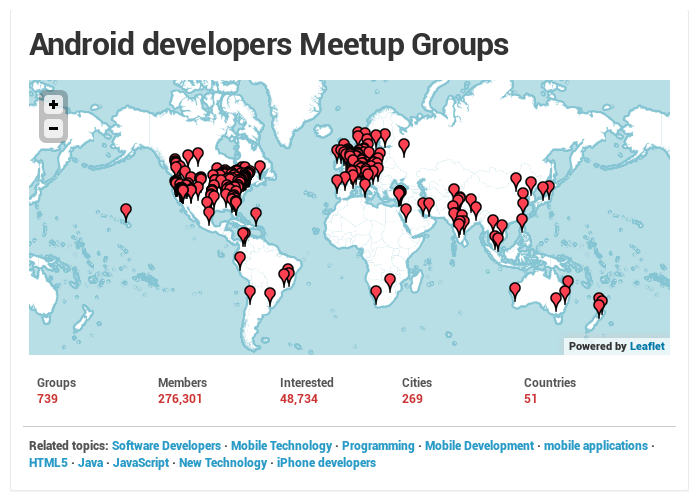
\includegraphics{android-meetups.png}}
\note{locality matters}

\takahashi{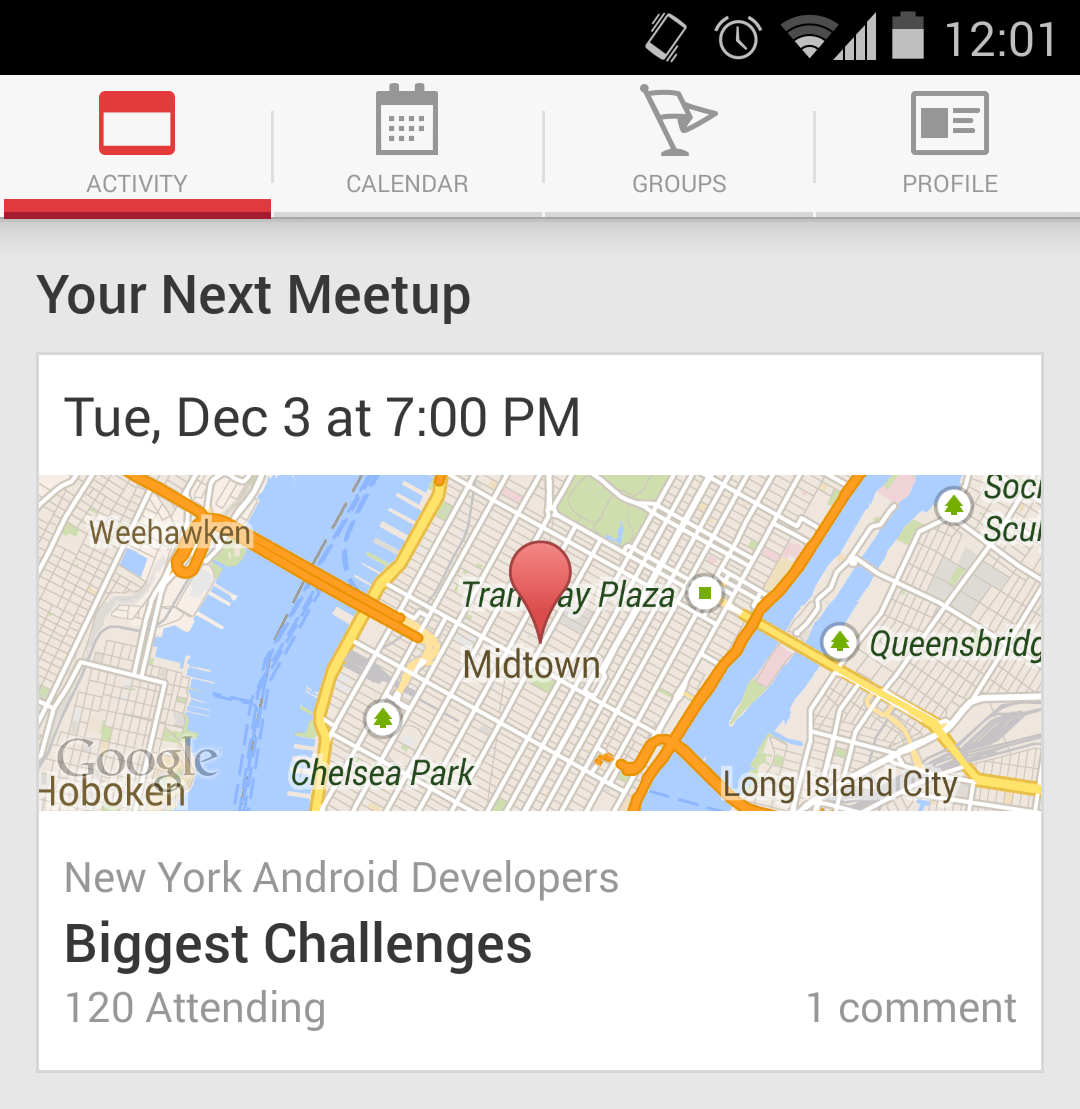
\includegraphics{mup-for-android.png}}
\note{personalization matters}

\begin{frame}
\frametitle{Stay in touch}
\begin{itemize}
\item Email: \texttt{mlc@meetup.com}
\item Twitter: \texttt{@vermicelli}
\end{itemize}
\end{frame}
\end{document}
